%\title{University of Bristol Thesis Template}
\RequirePackage[l2tabu]{nag}		% Warns for incorrect (obsolete) LaTeX usage
%
%
% File: memoirthesis.tex
%%%%%%%%%%%%%%%%%%%%%%%%%%%%%%%%%%%%
% Adapted for the MSc Robotics at University of Bristol and University of the West of England
%%%%%%%%%%%%%%%%%%%%%%%%%%%%%%%%%%%%
% Author: Victor Brena
% Description: Contains the thesis template using memoir class,
% which is mainly based on book class but permits better control of 
% chapter styles for example. This template is an adaptation and 
% modification of Oscar's.
% 
% Memoir is a flexible class for typesetting poetry, fiction, 
% non-fiction and mathematical works as books, reports, articles or
% manuscripts. CTAN repository is found at:
% http://www.ctan.org/tex-archive/macros/latex/contrib/memoir/
%
%
% UoB guidelines for thesis presentation were found at:
% http://www.bris.ac.uk/esu/pg/pgrcop11-12topic.pdf#page=49
%
% UoB guidelines:
%
% The dissertation must be printed on A4 white paper. Paper up to A3 may be used
% for maps, plans, diagrams and illustrative material. Pages (apart from the
% preliminary pages) should normally be double-sided.
%
% Memoir class loads useful packages by default (see manual).
\documentclass[a4paper,11pt,reqno,openbib,oldfontcommands, oneside]{memoir} %add 'draft' to turn draft option on (see below)
%
%
% Adding metadata:
\usepackage{datetime}
\usepackage{ifpdf}
\ifpdf
\pdfinfo{
   /Author (Author's name)
   /Title (MSc Thesis)
   /Keywords (One; Two;Three)
   /CreationDate (D:\pdfdate)
}
\fi
% When draft option is on. 
\ifdraftdoc 
	\usepackage{draftwatermark}				%Sets watermarks up.
	\SetWatermarkScale{0.3}
	\SetWatermarkText{\bf Draft: \today}
\fi
%
% Declare figure/table as a subfloat.
\newsubfloat{figure}
\newsubfloat{table}
% Better page layout for A4 paper, see memoir manual.
\settrimmedsize{297mm}{210mm}{*}
\setlength{\trimtop}{0pt} 
\setlength{\jot}{10pt}
\setlength{\trimedge}{\stockwidth} 
\addtolength{\trimedge}{-\paperwidth} 
\settypeblocksize{634pt}{448.13pt}{*} 
\setulmargins{4cm}{*}{*} 
\setlrmargins{*}{*}{1.5} 
\setmarginnotes{17pt}{51pt}{\onelineskip} 
\setheadfoot{\onelineskip}{2\onelineskip} 
\setheaderspaces{*}{2\onelineskip}{*} 
\checkandfixthelayout
%
\frenchspacing
% Font with math support: New Century Schoolbook
\usepackage{fouriernc}
\usepackage[T1]{fontenc}
%
% UoB guidelines:
%
% Text should be in double or 1.5 line spacing, and font size should be
% chosen to ensure clarity and legibility for the main text and for any
% quotations and footnotes. Margins should allow for eventual hard binding.
%
% Note: This is automatically set by memoir class. Nevertheless \OnehalfSpacing 
% enables double spacing but leaves single spaced for captions for instance. 
\OnehalfSpacing 
%
% Sets numbering division level
\setsecnumdepth{subsection} 
\maxsecnumdepth{subsubsection}
%
% Chapter style (taken and slightly modified from Lars Madsen Memoir Chapter 
% Styles document
\usepackage{calc,soul,fourier}
\makeatletter 
\newlength\dlf@normtxtw 
\setlength\dlf@normtxtw{\textwidth} 
\newsavebox{\feline@chapter} 
\newcommand\feline@chapter@marker[1][4cm]{%
	\sbox\feline@chapter{% 
		\resizebox{!}{#1}{\fboxsep=1pt%
			\colorbox{gray}{\color{white}\thechapter}% 
		}}%
		\rotatebox{90}{% 
			\resizebox{%
				\heightof{\usebox{\feline@chapter}}+\depthof{\usebox{\feline@chapter}}}% 
			{!}{\scshape\so\@chapapp}}\quad%
		\raisebox{\depthof{\usebox{\feline@chapter}}}{\usebox{\feline@chapter}}%
} 
\newcommand\feline@chm[1][4cm]{%
	\sbox\feline@chapter{\feline@chapter@marker[#1]}% 
	\makebox[0pt][c]{% aka \rlap
		\makebox[1cm][r]{\usebox\feline@chapter}%
	}}
\makechapterstyle{daleifmodif}{
	\renewcommand\chapnamefont{\normalfont\Large\scshape\raggedleft\so} 
	\renewcommand\chaptitlefont{\normalfont\Large\bfseries\scshape} 
	\renewcommand\chapternamenum{} \renewcommand\printchaptername{} 
	\renewcommand\printchapternum{\null\hfill\feline@chm[2.5cm]\par} 
	\renewcommand\afterchapternum{\par\vskip\midchapskip} 
	\renewcommand\printchaptertitle[1]{\color{gray}\chaptitlefont\raggedleft ##1\par}
} 
\makeatother 
\chapterstyle{daleifmodif}
%
% UoB guidelines:
%
% The pages should be numbered consecutively at the bottom centre of the
% page.
\makepagestyle{myvf} 
\makeoddfoot{myvf}{}{\thepage}{} 
\makeevenfoot{myvf}{}{\thepage}{} 
\makeheadrule{myvf}{\textwidth}{\normalrulethickness} 
\makeevenhead{myvf}{\small\textsc{\leftmark}}{}{} 
\makeoddhead{myvf}{}{}{\small\textsc{\rightmark}}
\pagestyle{myvf}
%
% Oscar's command (it works):
% Fills blank pages until next odd-numbered page. Used to emulate single-sided
% frontmatter. This will work for title, abstract and declaration. Though the
% contents sections will each start on an odd-numbered page they will
% spill over onto the even-numbered pages if extending beyond one page
% (hopefully, this is ok).
\newcommand{\clearemptydoublepage}{\newpage{\thispagestyle{empty}\cleardoublepage}}
%
%
% Creates indexes for Table of Contents, List of Figures, List of Tables and Index
\makeindex
% \printglossaries below creates a list of abbreviations. \gls and related
% commands are then used throughout the text, so that latex can automatically
% keep track of which abbreviations have already been defined in the text.
%
% The import command enables each chapter tex file to use relative paths when
% accessing supplementary files. For example, to include
% chapters/brewing/images/figure1.png from chapters/brewing/brewing.tex we can
% use
% \includegraphics{images/figure1}
% instead of
% \includegraphics{chapters/brewing/images/figure1}
\usepackage{import}

% Add other packages needed for chapters here. For example:
\usepackage{lipsum}					%Needed to create dummy text
\usepackage{amsfonts} 					%Calls Amer. Math. Soc. (AMS) fonts
\usepackage[centertags]{amsmath}			%Writes maths centred down
\usepackage{stmaryrd}					%New AMS symbols
\usepackage{amssymb}					%Calls AMS symbols
\usepackage{amsthm}					%Calls AMS theorem environment
\usepackage{newlfont}					%Helpful package for fonts and symbols
\usepackage{layouts}					%Layout diagrams
\usepackage{listings}
\usepackage{graphicx}					%Calls figure environment
\usepackage{longtable,rotating}			%Long tab environments including rotation. 
\usepackage[utf8]{inputenc}			%Needed to encode non-english characters 
\usepackage{pdfpages}
									%directly for mac
\usepackage{caption}
\usepackage{subcaption}
\usepackage{colortbl}					%Makes coloured tables
\usepackage{wasysym}					%More math symbols
\usepackage{mathrsfs}					%Even more math symbols
\usepackage{float}						%Helps to place figures, tables, etc. 
\usepackage{verbatim}					%Permits pre-formated text insertion
\usepackage{upgreek }					%Calls other kind of greek alphabet
\usepackage{latexsym}					%Extra symbols
\usepackage[square,numbers,
		     sort&compress]{natbib}		%Calls bibliography commands 
\usepackage{url}						%Supports url commands
% \usepackage{etex}						%eTeXÕs extended support for counters
% \usepackage{fixltx2e}					%Eliminates some in felicities of the 
									%original LaTeX kernel
\usepackage[spanish,english]{babel}		%For languages characters and hyphenation
\usepackage{color}                    				%Creates coloured text and background
\usepackage[colorlinks=true,
		     allcolors=black]{hyperref}              %Creates hyperlinks in cross references
\usepackage{memhfixc}					%Must be used on memoir document 
									%class after hyperref
\usepackage{enumerate}					%For enumeration counter
\usepackage{footnote}					%For footnotes
\usepackage{microtype}					%Makes pdf look better.

\usepackage{rotfloat}					%For rotating and float environments as tables, 
									%figures, etc. 
\usepackage{alltt}						%LaTeX commands are not disabled in 
									%verbatim-like environment
\usepackage[version=0.96]{pgf}			%PGF/TikZ is a tandem of languages for producing vector graphics from a 
\usepackage{tikz}						%geometric/algebraic description.
\usetikzlibrary{arrows,shapes,snakes,
		       automata,backgrounds,
		       petri,topaths,calc, positioning}				%To use diverse features from tikz		
%							
%Reduce widows  (the last line of a paragraph at the start of a page) and orphans 
% (the first line of paragraph at the end of a page)
\widowpenalty=1000
\clubpenalty=1000
%
% New command definitions for my thesis
%
\newcommand{\keywords}[1]{\par\noindent{\small{\bf Keywords:} #1}} %Defines keywords small section
\newcommand{\parcial}[2]{\frac{\partial#1}{\partial#2}}                             %Defines a partial operator
\newcommand{\vectorr}[1]{\mathbf{#1}}                                                        %Defines a bold vector
\newcommand{\vecol}[2]{\left(                                                                         %Defines a column vector
	\begin{array}{c} 
		\displaystyle#1 \\
		\displaystyle#2
	\end{array}\right)}
\newcommand{\mados}[4]{\left(                                                                       %Defines a 2x2 matrix
	\begin{array}{cc}
		\displaystyle#1 &\displaystyle #2 \\
		\displaystyle#3 & \displaystyle#4
	\end{array}\right)}
\newcommand{\pgftextcircled}[1]{                                                                    %Defines encircled text
    \setbox0=\hbox{#1}%
    \dimen0\wd0%
    \divide\dimen0 by 2%
    \begin{tikzpicture}[baseline=(a.base)]%
        \useasboundingbox (-\the\dimen0,0pt) rectangle (\the\dimen0,1pt);
        \node[circle,draw,outer sep=0pt,inner sep=0.1ex] (a) {#1};
    \end{tikzpicture}
}
\newcommand{\range}[1]{\textnormal{range }#1}                                             %Defines range operator
\newcommand{\innerp}[2]{\left\langle#1,#2\right\rangle}                                 %Defines inner product
\newcommand{\prom}[1]{\left\langle#1\right\rangle}                                         %Defines average operator
\newcommand{\tra}[1]{\textnormal{tra} \: #1}                                                       %Defines trace operator
\newcommand{\sign}[1]{\textnormal{sign\,}#1}                                                   %Defines sign operator
\newcommand{\sech}[1]{\textnormal{sech} #1}                                                  %Defines sech
\newcommand{\diag}[1]{\textnormal{diag} #1}                                                    %Defines diag operator
\newcommand{\arcsech}[1]{\textnormal{arcsech} #1}                                       %Defines arcsech
\newcommand{\arctanh}[1]{\textnormal{arctanh} #1}                                         %Defines arctanh
%Change tombstone symbol
\newcommand{\blackged}{\hfill$\blacksquare$}
\newcommand{\whiteged}{\hfill$\square$}
\newcounter{proofcount}
\renewenvironment{proof}[1][\proofname.]{\par
 \ifnum \theproofcount>0 \pushQED{\whiteged} \else \pushQED{\blackged} \fi%
 \refstepcounter{proofcount}
 \normalfont 
 \trivlist
 \item[\hskip\labelsep
       \itshape
   {\bf\em #1}]\ignorespaces
}{%
 \addtocounter{proofcount}{-1}
 \popQED\endtrivlist
}
%
%
% New definition of square root:
% it renames \sqrt as \oldsqrt
\let\oldsqrt\sqrt
% it defines the new \sqrt in terms of the old one
\def\sqrt{\mathpalette\DHLhksqrt}
\def\DHLhksqrt#1#2{%
\setbox0=\hbox{$#1\oldsqrt{#2\,}$}\dimen0=\ht0
\advance\dimen0-0.2\ht0
\setbox2=\hbox{\vrule height\ht0 depth -\dimen0}%
{\box0\lower0.4pt\box2}}
%
% My caption style
\newcommand{\mycaption}[2][\@empty]{
	\captionnamefont{\scshape} 
	\changecaptionwidth
	\captionwidth{0.9\linewidth}
	\captiondelim{.\:} 
	\indentcaption{0.75cm}
	\captionstyle[\centering]{}
	\setlength{\belowcaptionskip}{10pt}
	\ifx \@empty#1 \caption{#2}\else \caption[#1]{#2}
}
%
% My subcaption style
\newcommand{\mysubcaption}[2][\@empty]{
	\subcaptionsize{\small}
	\hangsubcaption
	\subcaptionlabelfont{\rmfamily}
	\sidecapstyle{\raggedright}
	\setlength{\belowcaptionskip}{10pt}
	\ifx \@empty#1 \subcaption{#2}\else \subcaption[#1]{#2}
}
%
%An initial of the very first character of the content
\usepackage{lettrine}
\newcommand{\initial}[1]{%
	\lettrine[lines=3,lhang=0.33,nindent=0em]{
		\color{gray}
     		{\textsc{#1}}}{}}
%
% Theorem styles used in my thesis
%
\theoremstyle{plain}
\newtheorem{theo}{Theorem}[chapter]
\theoremstyle{plain}
\newtheorem{prop}{Proposition}[chapter]
\theoremstyle{plain}
\theoremstyle{definition}
\newtheorem{dfn}{Definition}[chapter]
\theoremstyle{plain}
\newtheorem{lema}{Lemma}[chapter]
\theoremstyle{plain}
\newtheorem{cor}{Corollary}[chapter]
\theoremstyle{plain}
\newtheorem{resu}{Result}[chapter]
%
% Hyphenation for some words
%
\hyphenation{res-pec-tively}
\hyphenation{mono-ti-ca-lly}
\hyphenation{hypo-the-sis}
\hyphenation{para-me-ters}
\hyphenation{sol-va-bi-li-ty}
%
%
\begin{document}
% UoB guidlines:
%
% Preliminary pages
% 
% The five preliminary pages must be the Title Page, Abstract, Dedication
% and Acknowledgements, Author's Declaration and Table of Contents.
% These should be single-sided.
% 
% Table of contents, list of tables and illustrative material
% 
% The table of contents must list, with page numbers, all chapters,
 % sections and subsections, the list of references, bibliography, list of
% abbreviations and appendices. The list of tables and illustrations
% should follow the table of contents, listing with page numbers the
% tables, photographs, diagrams, etc., in the order in which they appear
% in the text.
% 
\frontmatter
\pagenumbering{roman}
%
\begin{titlingpage}
\begin{SingleSpace}
\calccentering{\unitlength} 
\begin{adjustwidth*}{\unitlength}{-\unitlength}
\vspace*{13mm}
\begin{center}
\rule[0.5ex]{\linewidth}{2pt}\vspace*{-\baselineskip}\vspace*{3.2pt}
\rule[0.5ex]{\linewidth}{1pt}\\[\baselineskip]
{\HUGE Converge}\\[4mm]
{\Large \textit{A business blockchain for sophisticated asset management and cross-business transactions}}\\
\rule[0.5ex]{\linewidth}{1pt}\vspace*{-\baselineskip}\vspace{3.2pt}
\rule[0.5ex]{\linewidth}{2pt}\\
\vspace{6.5mm}
{\large By}\\
\vspace{6.5mm}
{\large\textsc{Alex Greig}}\\
\vspace{10mm}

\includegraphics[scale=0.15]{logos/sta.png}
\\
\vspace{10mm}
{\large Software Design and Development - Task 3\\
\textsc{St Augustine's College}} \\

\vspace{11mm}
\begin{minipage}{13cm}
	\center A project proposal to Big Time Software for the development of \textit{Converge}. A business blockchain that utilises an intelligent consensus mechanism and concepts such as tokenisation, converge will efficiently create a complete, transparent, tamperproof history and facilitation of the information flows, inventory flows, and financial flows in transactions.
\end{minipage}\\
\vspace{9mm}
{\large\textsc{23 June 2022}}
\vspace{12mm}
\end{center}
\begin{flushright}
%{\small Word count: ten thousand and four}
\end{flushright}
\end{adjustwidth*}
\end{SingleSpace}
\end{titlingpage}

\clearemptydoublepage
%
\renewcommand{\contentsname}{Table of Contents}
\maxtocdepth{subsection}
\tableofcontents*
\addtocontents{toc}{\par\nobreak \mbox{}\hfill{\bf Page}\par\nobreak}
\clearemptydoublepage
%

% The bulk of the document is delegated to these chapter files in
% subdirectories.
\mainmatter
%
\let\textcircled=\pgftextcircled
\chapter{Problem Definition}
\label{chap:intro}

\initial{R}esurfacing after the tribulations of COVID-19, travel is becoming more prominent than ever as people from all around the world wish to explore and experience the world. Planning and organising holidays has always been time consuming, stressful and confusing. Traverse is a sophisticated travel application that utilises machine learning to enable the user to develop a personalised itinerary within a target budget; and discover and book different transport, activities, restaurants and hotels based off independent reviews and ratings. Complementing the rating system, which is not completed by all travellers, the artificial intelligence will build profiles of different businesses and the frequency and polarity of visits and use that to recommend different activities. The mobile application allows users to store photos within the holiday timeline on their profile and share their experiences with only friends or the public domain. The user can also get inspiration for holiday ideas from friends and family, or the wider community of individuals and groups who travel the world. \\

Through answering a small number of questions, such as the priorities of travelling (food, culture, adrenaline inducing experiences), the machine learning model will recommend activities associated with a certain destination to the user, allowing for discovery of new places easily and efficiently. Another issue that is prevalent when travelling is the struggle in trying to book accommodation and flights, and the dilemma of which one to book first. Traverse will solve this problem, through simultaneous booking, enabling the user to book both the flights and accommodation without stressing over availability. In conjunction to this, the artificial intelligence will ensure that their is no overlaps in the schedule or excess waiting time for transportation, such as connecting flights, so that the travelling experience will be seamless. Thus the machine learning will use the user preferences, budget, time frame and destination to efficiently build a personalised itinerary. \\

The mobile application will give the user the ability to use flight numbers to retrieve flight information from the International Air Transport Association (IATA) and the International Civil Aviation Organization (ICAO) API which can then be input into the itinerary so that all the updated times and locations of each event, for example delayed flights, are in one place. The application will also use bus, ferry and train timetables to specify in their schedule the different options the user can use to get between each location, highlighting the most time and cost effective. Therefore, the traditional approach of navigating through websites and convoluted booking sites to try and plan travel is significantly improved by Traverse, as all aspects of planning travel are located in one application, allowing smooth travel that will lead to new experiences and adventures.




\clearemptydoublepage

\let\textcircled=\pgftextcircled
\chapter{Issues Relevant to Program}

\initial{B}lockchain is an open digital ledger technology that has the capability of significantly altering the way that people operate in organizations. Blockchain’s ethical issues for business catalyse from its three main promises: immutability, disintermediation, and automation. Immutability results in the permanency of a human past record and raises ethical issues such as privacy and transparency concerns. Disintermediation refers to horizontal decision-making and the numerosity of stakeholders in verifying outcomes which raises ethical issues related to accountability and equal opportunity. Automation refers to the self-executing features of coded agreements called smart contracts which raises issues related to the absence of human decision making and the inability for human intervention. The main ethical issue that will be discussed, however, is the inadvertent asymmetry of power that is being created, as large corporations have access to more bargaining power, information, and efficient transactions then smaller possibly local businesses. \\

In this sense, this business blockchain might enable transactions that are the product of force or possibly even fraudulent activity that would normally be prevented through institutions such as banks or government bodies. These mediating institutions would normally identify and constrain the misuse of markets by large corporations, however, by managing their assets and transactions through the business blockchain, this might be circumvented. This would enable different types of illegal and immoral transactions by facilitating transactions without intermediaries who can personally be held accountable for those transactions. \\

A case in point is the “assassination markets.” AUGUR is an Ethereum-based blockchain application for the creation of “peer-to-peer prediction markets” which allow people to place bets secretly. AUGUR has created, invertedly, a utilisation of blockchain analogous to the “assassination market” in that it allows anonymous betting upon someone's death, which in turn may incentivize people to kill others so as to win these very bets. \\

Although this real-world example is slightly disconnected from business blockchains the same unintended use cases of the software may occur. The actualisation of this ethical issue in this business blockchain may come in the form of businesses trading slave labour that breaks jurisdiction regarding minimum wages and the fair work rights, however, due to the transaction being mediated through blockchain technology, the unethical actions might go unnoticed.

\clearemptydoublepage
\let\textcircled=\pgftextcircled
\chapter{Context and Dataflow Diagrams}

\section{Context Diagram}

\vspace{2cm}
\begin{figure}[H]
\caption{Context Diagram}
\vspace{1cm}
\centering
\begin{tikzpicture}[
roundnode/.style={circle, scale = 1.2, draw=green!60, fill=green!5, very thick, minimum size=7mm},
squarednode/.style={rectangle, scale = 1.2, draw=red!60, fill=red!5, very thick, minimum size=5mm},
to/.style={->,>=stealth,shorten >=1pt,semithick},
]
%nodes
\node[squarednode](e1) at (-6, 2) {User};
\node[roundnode](p) at (0,0) {Traverse};
\node[squarednode](e2) at (6, 2) {Businesses Database};
\node[squarednode](e3) at (-6, -2) {Flight / Transportation APIs};
\node[squarednode](e4) at (6, -2) {User's Database};
%connections
\draw[to] (e1) to [bend left = 16] node[align=center, text width = 4cm, above = 0cm, rotate=-25] {Account, Budget, Selections}(p);
\draw[to] (p) to [bend left = 16] node[align=center,text width = 4cm, pos=0.8, below = 0cm, rotate=-25] {Recommendations, Itinerary}(e1);
\draw[to] (p) to [bend left = 16] node[align=center,text width = 4cm, midway, above = 0cm, rotate=25] {Location of interest, Category}(e2);
\draw[to] (e2) to [bend left = 16] node[align=center,text width = 4cm, pos=0.2, below = 0cm, rotate=25] {Ratings, Business Availabilities}(p);
\draw[to] (e3) to [bend left = 16] node[align=center, text width = 4cm, above = 0cm, pos=0.15, rotate=25] {Transportation Information}(p);
\draw[to] (p) to [bend left = 16] node[align=center,text width = 4cm, midway, below = 0cm, rotate=25] {Time, Location, Destination}(e3);
\draw[to] (p) to [bend left = 16] node[align=center,text width = 4cm, pos=0.85, above = 0cm, rotate=-25] {Login Details}(e4);
\draw[to] (e4) to [bend left = 16] node[align=center,text width = 4cm, midway, below = 0cm, rotate=-25] {User Profile, Preferences, Personalised Itinerary}(p);
\end{tikzpicture}
\end{figure}

\section{Data Flow Diagram - Core Functionality}
\begin{figure}[H]
\caption{Data Flow Diagram - Core Functionality}
\vspace{0.3cm}
\centering
\begin{tikzpicture}[node distance = 2.5cm,
process/.style={circle, scale = 0.8, align=center, text width = 2cm, draw=green!60, fill=green!5, very thick, minimum size=7mm},
entity/.style={rectangle, scale = 1.2, align=center, text width = 2cm, draw=red!60, fill=red!5, very thick, minimum size=5mm},
path/.style={->,>=stealth,shorten >=1pt,semithick},
]

\tikzset{
  pics/datastore/.style args={#1,#2, #3}{
     code={
	     \draw [draw=blue!60] (0,0) -- (3,0) -- (3,1) -- (0, 1);
	     \node[#3] (#1) at (1.5,0.5) {#2};
     }
  }
}

%Nodes
\node [entity] (user) {User};
\node [process] (login) [below left = of user]{Login};
\node [process] (signup) [below right = of user]{Signup};
\node [process] (ansqs) [below = of signup, xshift=1cm]{Answer Preference Questions};
\draw (-1.5, -6) pic{datastore={ud1, User Database, black}};
\node [process] (loadint) [below = of login, xshift= -1cm]{Load Itinerary};
\node [process] (mlig) [below = of ud1]{Machine Learning Itinerary Generation};
\node [process] (conf) [below = of mlig]{Confirm Booking};
\node [entity, yshift= 0cm, xshift = 0.7cm] (user1) [below = of conf]{User};
\draw (3.5, -11) pic{datastore={ft1, Transport APIs, black}};
\draw (-6.5, -11) pic{datastore={e1, Events Database, black}};
\node [process] (add) [below = of e1]{Add Events and Update Availabilities};
\node [scale =0.9, yshift = -3.5cm, xshift = -3cm, align=center, draw=red!60, fill=red!5, very thick] (u1) at (add) {Businesses};
\node [scale = 1, yshift = -1cm, xshift = 2cm, align=center, draw=red!60, fill=red!5, very thick] (u2) at (u1) {...};
\node [scale =0.9, yshift = 1 cm, xshift = 3cm, align=center, draw=red!60, fill=red!5, very thick] (u3) at (u2) {Another Business};
\node [process, yshift = 1cm] (change) [below = of ft1]{Search and Change Events / Customise};
\node [process, yshift = 1cm] (iti) [below = of change]{Show Itinerary, Updates};

% Paths
\draw [stealth-stealth, semithick](user) edge[out=200, in=90] node[align=center, midway, text width=2.5cm, above = 0.2cm] {Login Details} node[align=center, pos=0.3, text width=2.5cm, below = 0.2cm] {Success Flag} (login); 
\draw [stealth-stealth, semithick] (login) to node[align=center, text width=2.5cm, midway, rotate = -35, above] {Login Details} node[align=center, text width=2.5cm, midway, rotate = -35, below] {Validation} ($(login)!3.5cm!(ud1)$); 
\draw [stealth-stealth, semithick] (signup) to node[align=center, text width=2.5cm, midway, rotate = 35, above] {Signup Details, Profile Visibility} node[align=center, text width=2.5cm, midway, rotate = 35, below] {Validation} ($(signup)!3.5cm!(ud1)$); 
\draw [stealth-stealth, semithick](user) edge[out=340, in=90] node[align=center, midway, text width=2.5cm, above = 0.2cm] {Profile Visibility, Signup Details} node[align=center, pos=0.3, text width=2.5cm, below= 0.2cm] {Success Flag} (signup); 
\draw [path](login) edge[out=210, in=120] (loadint); 
\draw [path](signup) edge[out=330, in=60] (ansqs); 
\draw [stealth-stealth, semithick] (loadint) to node[align=center, text width=2.5cm, midway, rotate = 20, above] {Personalised Itinerary} node[align=center, text width=2.5cm, midway, rotate = 20, below] {Username} ($(loadint)!3.3cm!(ud1)$); 
\draw [path] (ansqs) to node[align=center, text width=2.5cm, midway, rotate = -20, above] {Username, Preferences} ($(ansqs)!3.3cm!(ud1)$); 
\draw [path, shorten <= 0.3cm] (ud1) to node[align=center, text width=2.5cm, midway, rotate = 90, above] {Username, Preferences} (mlig);
\draw [stealth-stealth, semithick] (mlig) to node[align=center, text width=2.5cm, midway, rotate = -10, above] {Location, Destination, Budget} node[align=center, text width=2.5cm, midway, rotate = -10, below] {Transport Available, Delayed Flights}($(mlig)!3.5cm!(ft1)$); 
\draw [stealth-stealth, semithick] (mlig) to node[align=center, text width=2.5cm, midway, rotate = 10, above] {User Preferences, Location} node[align=center, text width=2.5cm, midway, rotate = 10, below] {Events}($(mlig)!3.5cm!(e1)$); 
\draw [dashed](u1) -- (u2);
\draw [dashed](u2) -- (u3);
\draw [dashed](u1) -- (u3);
\draw [path] (u1) to [bend left = 30](add.210); 
\draw [path] (u2) to node[align=center, text width=2.5cm, midway, above, xshift=-1cm] {Events, Updates} node[align=center, text width=2.5cm, midway, above, xshift=1cm] {Events, Updates}(add); 
\draw [path] (u3) to [bend right = 30] (add.330); 
\draw [path, shorten >= 0.3cm] (add) to node[align=center, text width=2.5cm, midway, rotate = 90, above] {Events} (e1);
\draw [stealth-stealth, semithick] (user1) to node[align=center, text width=2.5cm, pos=0.53, above, rotate=-77] {Confirmation, Payment} node[align=center, text width=2.5cm, midway, below, rotate=-77] {Success Flag}(conf); 
\draw [path] (mlig) to node[align=center, text width=2.5cm, midway, rotate = 90, above] {Personalised Itinerary} (conf);
\draw [path] (iti) to node[align=center, text width=2.5cm, midway, above] {Updates} (user1); 
\draw [stealth-stealth, semithick] (user1) to node[align=center, text width=2.5cm, pos=0.6, rotate = 45, above] {Search, Location} node[align=center, text width=2.5cm, pos=0.6, rotate = 45, below] {Events, Availabilities}(change); 

\end{tikzpicture}

\end{figure}


\section{Data Flow Diagram - Social Functionality}
\begin{figure}[H]
\caption{Data Flow Diagram - Social Functionality}
\vspace{1cm}
\centering
\begin{tikzpicture}[node distance = 2.5cm,
process/.style={circle, scale = 0.8, align=center, text width = 2cm, draw=green!60, fill=green!5, very thick, minimum size=7mm},
entity/.style={rectangle, scale = 1.2, align=center, text width = 2cm, draw=red!60, fill=red!5, very thick, minimum size=5mm},
path/.style={->,>=stealth,shorten >=1pt,semithick},
]

\tikzset{
  pics/datastore/.style args={#1,#2, #3}{
     code={
	     \draw [draw=blue!60] (0,0) -- (3,0) -- (3,1) -- (0, 1);
	     \node[#3] (#1) at (1.5,0.5) {#2};
     }
  }
}

% Nodes
\node [entity] (user) {User};
\node [process] (sub) [below left = of user]{Submit Photos and Ratings of Events};
\node [process] (exp) [below right = of user]{Explore Friends Profiles and Holidays};
\draw (-1.5, -6.5) pic{datastore={ud1, User Database, black}};
\node [process] (copy) [below = of ud1]{Copy Friends Events / Itinerary};

% Paths
\draw [path] (user) to node[align=center, text width=2.5cm, midway, rotate = 40, above] {Photos, Ratings} (sub); 
\draw [stealth-stealth, semithick] (user) to node[align=center, text width=2.5cm, midway, rotate = -40, above] {Friend's Username} node[align=center, text width=2.5cm, midway, rotate = -40, below] {Friend's Profile and Holidays} (exp); 
\draw [path, shorten >= 0.5cm] (sub) to node[align=center, text width=2.5cm, pos=0.5, above, rotate=-40] {Photos, Ratings} (ud1);
\draw [stealth-stealth, semithick, shorten >= 0.5cm] (exp) to node[align=center, text width=2.5cm, pos=0.4, above, rotate=40] {Username} node[align=center, text width=2.5cm, pos=0.4, below, rotate=40] {Profile, Past Itinerary} (ud1);
\draw [path, shorten >= 0.5cm] (copy) to node[align=center, text width=2.5cm, pos=0.5, above, rotate=90] {Itinerary, Username} (ud1);
\draw [path](exp) edge[out=290, in=70] node[align=center, text width=2.5cm, pos=0.5, below, rotate=30] {Friend's Holiday} (copy); 
\end{tikzpicture}
\end{figure}

\clearemptydoublepage
\let\textcircled=\pgftextcircled
\chapter{Algorithms}
\renewcommand{\ttdefault}{pcr}
\lstset{
	basicstyle=\small\ttfamily,
	captionpos=t,
	numbers=left,
	tabsize=4,
	keywordstyle=\bfseries,
	breaklines=true,
	columns=fullflexible,
	numbersep=-8pt, 
	frame = shadowbox,
	morekeywords={BEGIN, END, DISPLAY, INPUT, IF, ENDIF, WHILE, DO, ELSE, THEN, OR, OPEN, RETURN, WRITE, NEXT, FOR, APPEND, CLOSE, PASS, AND, OUTPUT}
}

The core algorithms that will be used in the application are displayed below, written in the pseudo-code syntax:

\section{Main Program}

\begin{lstlisting}[caption=Main Program, escapechar=\@]
	BEGIN MAINPROGRAM
		@\underline{LoadLandingPage()}@ // Instantiates the program and loads the landing page with buttons for the user's selection.
		IF SignUp.pressed() == True THEN
			@\underline{LoadSignUp()}@ // Loads the sign up 
			INPUT username, password, email, confirm_password
			IF username.entered() == True AND email.entered() == True AND password.entered() == True AND password == confirm_password THEN
				IF username.validate() == True AND password.validate() == True THEN
					Display tickIcon
					@\underline{SendValidationEmail()}@ // Sends a validation email to the email address that was inputted by the user, so that it can be verified.
					Display "Verification Email Sent!"
					@\underline{LoadPreferences()}@ // Loads the first question and the associated input sliders within them.
					WHILE question <> last_question DO
						INPUT answer // Answer is inputted through slider so the answer will be a float.
						IF next_question.pressed() == True AND question_answered() THEN
							@\underline{LoadNextQuestion()}@
							@\underline{UpdateUserData(question, username, answer)}@ // Data will be entered into the database based upon the type of data so that the machine learning model can use the information to predict recommendations that the user will like. This is done so that this function can be reused to update the User Profile Database.

						ELSE IF skip_question.pressed() == True THEN  
							@\underline{LoadNextQuestion()}@
						ENDIF
					ENDWHILE

					INPUT answer // Answer is inputted through slider so the answer will be a float.
					IF next_question.pressed() == True AND question_answered() THEN
						@\underline{UpdateUserData(username, question, answer)}@
					ENDIF
					@\underline{LoadTripPlanning()}@
					INPUT budget, from, to, duration, group_size // from and to are the beginning and ending destinations.
					business_records = @\underline{ReadBusinessData()}@ // Interacts with Business Database and reads the availabilities and different business events into memory.
					user_data = @\underline{ReadUserData()}@ // Reads user data into memory to input into the machine learning model for recommending and optimising itinerary.
					transport_data = @\underline{TransportAPI(duration)}@ //Retrives transport data within the duration period which can be used to decide the method of transport between locations when travelling.
					ml_input_data = business_records, user_data, budget, from, to, duration, group_size, transport_data // Data that the machine learning model will use to make sophisiticated decisions about events to recommend the user. This datatype is a tuple as it contains multiple different datatypes.
					ml_recommendations = @\underline{MachineLearningRecomendations(ml\_input\_data)}@
					@\underline{LoadFlights(ml\_recommendations)}@ // Parameters of the function are the ml recommendations as these recommendations will then be loaded for the user.
					INPUT flights_chosen
					@\underline{UpdateUserData("Flights", username, flights\_chosen)}@ //Parameters are the dataID, data and the username of the User.

					@\underline{LoadHotels(ml\_recommendations)}@
					INPUT hotels_chosen
					@\underline{UpdateUserData("Hotels", username, hotels\_chosen)}@

					@\underline{LoadActivities(ml\_recommendations)}@
					INPUT activities_chosen
					@\underline{UpdateUserData("Activities", username, activities\_chosen)}@

					@\underline{LoadDiscover()}@ // Loads the discover page which lets the user customise their itinerary.
					INPUT extra_activities
					@\underline{UpdateUserData("Activites", username, extra\_activities)}@

					@\underline{LoadPayment()}@ 
					INPUT payment_method
					@\underline{ConcurrentBooking(payment\_method, user\_data)}@
					DISPLAY Success

					@\underline{HomeItinerary()}@ // Function that loads the itinerary and other options for the user. This will take the user to the main page and enable them to explore other activities, look at their flights and interact with the social options of the mobile application.

				ELSE
					Display crossIcon
				ENDIF
			ENDIF
			IF username.entered() == True THEN
				If username.validate() == True THEN
					Display tickIcon
				ELSE
					Display crossIcon
				ENDIF
			ENDIF
		ELSE IF SignIn.pressed() == True THEN
			@\underline{LoadSignIn()}@ // Loads the sign in functionality
			IF username.entered() == True AND password.entered() THEN
				If username.validate() == True THEN
					Display tickIcon
					@\underline{HomeItinerary()}@ // Function that loads the itinerary and other options for the user. This will take the user to the main page and enable them to explore other activities, look at their flights and interact with the social options of the mobile application.

				ELSE
					Display crossIcon
				ENDIF
			ENDIF
		ENDIF

	END MAINPROGRAM

\end{lstlisting}

\section{Update User Data}

\begin{lstlisting}[caption=Update User Data, escapechar=\@]
	BEGIN  @\underline{UpdateUserData(dataID, username, data)}@
		OPEN UserDatabase for relative access
		dataIDs = array of identifiers of all questions // These should correlate to dataID passed into function when retrieving the user preferences.
		FOR i=0 to users.len() DO
			IF users[i].username == username THEN
				FOR i=0 to dataIDs.len() DO
					IF dataIDs[i] == dataID THEN
						WRITE UserData.users[i] from data using dataID	
					ENDIF
				NEXT i
			ENDIF
		NEXT i
		CLOSE UserDatabase
	END  @\underline{UpdateUserData}@
\end{lstlisting}

Machine learning algorithms in recommender systems are typically classified into two categories — content based and collaborative filtering methods although modern recommenders combine both approaches. Collaborative filtering looks for patterns in the user activity in relation to other users, to produce user specific recommendations whereas Content-based filtering recommends items with similar content (e.g. metadata, description, topics, keywords) to the items the user has liked or indicated to like in the past. \\

For this application the approach that would be taken based upon the preferences that are retrieved from the beginning would be a content-based filtering the user has indicated to some level their priorities when travelling and has given data through answering questions about preferences and other inputs such as budget. First the algorithm will find similarities between the events and activities within the business database and use the answers from the user to generate a similarity matrix. From this, the machine learning model will create Bayesian networks to model the links between the different events and the weightings of similarity, enabling recommendations to be made.

\section{Machine Learning Recommendations and Optimisation}

\begin{lstlisting}[caption=Machine Learning Recommendations and Optimisation, escapechar=\@]
	BEGIN  @\underline{MachineLearningRecomendations(ml\_input\_data)}@
		business_records, user_data, budget, from, to, duration, group_size, transport_data = ml_input_data // Data that the machine learning model will use to make sophisticated decisions about events to recommend the user. This is decompressing the tuple into multiple variables for utilisation.
		FOR i=0 to user_data.len() DO
			FOR j=0 to business_records.events.len() DO
				similarity_matrix[i][j] = cosine_similarity(user_data[i], budget, business_records.events[i]) // Constructs the similarity matrix based upon the similarity of user preferences and target budget with the different events.
			NEXT j
		NEXT i

		bayesian_network = @\underline{BayesianGeneration(similarity\_matrix, transport\_data)}@ //Transport data is used in the Bayesian network generation to link events not only by similarity and budget, but also the ability to be transported between the different locations.

		availabilities = business_records.availability
		recommendations = @\underline{GradientDescentOptimisation(availabilities,}@ @\underline{duration, user\_data, bayesian\_network)}@ //Optimisation of the timing of each event to make sure that the Itinerary lines up. Works by making steps towards a perfectly fitted timeslot by moving towards a minima and evaluating its performance based on a reward function. Utilises the events that are linked with the highest weighted similarity on the Bayesian network. 

		RETURN recommendation // Data type of recommendation is an event from business_records.events
		

	END  @\underline{MachineLearningRecomendations(ml\_input\_data)}@
			
\end{lstlisting}
\section{Interaction with Transport APIs}

\begin{lstlisting}[caption= Interaction with Transport APIs, escapechar=\@]
	BEGIN  @\underline{TransportAPI(duration)}@
		transport_services = multidimensional array of n elements of [transportID, api_key, query_address] // All the api_keys needed to access the APIs of different transportation APIs, the multidimensional array of 3 by n, is so that each api key is coupled with a transport ID and query address so that each transport service can be identified and queried.

		transport_data = empty multidimensional array // This array will contain each transport and the times of arrival and location for each transport service.
		FOR i=0 to transport_services.len() DO
			transport_data[i] = @\underline{HttpRequest(transport\_services[i][0],}@ @\underline{transport\_services[i][1], transport\_services[i][2])}@ 
		NEXT i
		RETURN transport_data
	END  @\underline{TransportAPI}@
\end{lstlisting}


\vfill{}

\clearemptydoublepage
\let\textcircled=\pgftextcircled
\chapter{Feasibility Study}
\section{Define The Problem}

Currently, businesses globally have to communicate across multiple departments and management systems to facilitate cross-company transactions, leading to costly mistakes, opaque interaction histories, high administration costs and long delays for the transference of capital to be processed. Business blockchains, an innovative solution to this global issue, are reinventing how transactions are managed. They can take time and costs out of almost any process, enabling near real-time operations. And they deliver a high degree of accuracy and control, with much less risk than many alternatives. Due to the immutable nature of the blockchain, a transparent record of all transactions is kept which can be utilised for bookkeeping and taxation purposes while also preventing fraudulent behaviour as all transactions are recorded and can be reproduced for litigious reasons. The business blockchain that is being created, therefore, will help supply chain partners and corporations globally by creating a complete, transparent, tamperproof history and facilitation of the information flows, inventory flows, and financial flows in transactions. This permissioned blockchain will outperform current enterprise resource planning solutions as it is able to manage all transactions extremely quickly and efficiently, through sharing the load of computation across all nodes in the blockchain. An example of the differences between conventional record keeping and blockchain for a transaction is shown below. \\

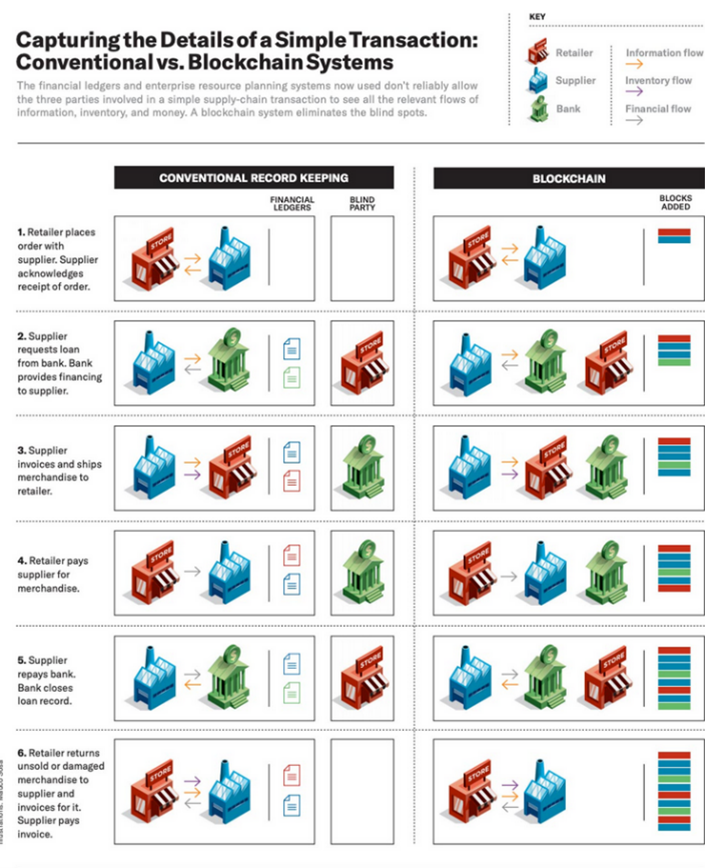
\includegraphics[width=\linewidth]{figures/vs.png} \\

The blockchain that is being developed is a proof of concept that will show the core functionality of permissioned blockchains and the benefits it produces. It will be compatible for all businesses as a node will be able to run on a server setup by the development team and users can interface with the system via a user-friendly web frontend to manage transactions and assets. The assets, labour and even items such as orders / invoices within each company will be tokenised on the blockchain so that businesses can interact with other businesses over the blockchain. Though it most commonly refers to the tokenization of financial or fungible assets, such as shares in a company or a quantity of gold, asset tokenization can hypothetically refer to the tokenization of any material or nonmaterial thing possessing monetary value: everything from a piece of art to a patent to an hour of a skilled worker’s time. This process of tokenization creates a bridge between real-world assets and their trading, storage and transfer in a digital world.\\

Although the functionality of transferring fungible and non-fungible assets will be implemented into the software solution, the legal processes surrounding the binding of assets will be implemented in the future. These legal proceedings are outside the scope of this project as they would require communication with governing institutions, intricate understanding of taxation law and connecting software solutions with the strenuous obligations of regulatory frameworks. \\

For the purpose of this conceptual design, I will utilise a main, “converge” token that is not truly backed by US Dollar or another asset, but in production, would be. The manner in which the tokens will be bound to physical assets is through the creation of a stable coin which reassures businesses will not have to consider the fluctuations of token value. To make this collateralised stable coin I would need to own the fiat or assets in which the token was based upon, as ‘collateral’ or conduct an exchange agreement with a bank in which the converge tokens could be converted into the local fiat currency. \\

\section{Economic Feasibility}
The economic feasibility of this project can be understood through a number of points of analysis. Firstly, the spending projection of the project needs to be addressed and how much working capital is required for the functioning of the software. Secondly, the cash flows need to be examined, including the revenues and the maintaining outflows of cash. \\

The spending projection for this project needs to be minimal as this scope of this project does not enable me to spend capital on expensive APIs, or high-end virtual private servers to host nodes for testing and compatibility studies. Thus, I have planned the project to use the most minimal costs possible as this fits within the boundaries of the project. I have utilised open-source frameworks to reduce costs and cut out any dependence on APIs. If this project was to be produced in reality, I would need to set aside ‘collateral’ in which the converge token was tied to so that it had a physical asset that it was bound to. This would be quite economically infeasible so a better method would be to conduct an exchange agreement with a bank in which the converge tokens could be converted into the local fiat currency. \\

The projected income expected from this project will come in the form of small fees that are collected on each transaction, although a small percentage, the sheer volume will make the process very economically advantageous. For example, a percentage for transaction such as 0.1\% will be a large incentive for continuing development and maintenance as if a trillion dollars passes through the network, that is around one billion dollars in revenue. If large volumes of transaction are occurring every day, then this will lead to a high profit. Further, as there are no central servers, the maintenance cost of the blockchain will be quite minimal, leading to lower expenditure and thus higher profits.

\section{Technical Feasibility}

Technical feasibility is the process of figuring out how you are going to produce your product or service to determine whether it is possible to create. Thus, with the aid of thorough research the software solution is feasible to create, however, it would require quite sophisticated technology that is only currently being developed. Firms around the globe are all attempting to understand and implement blockchain technology into their business, which reveals the pioneering needed to develop and implement such a software solution. Although it is technically feasible to create, the difficulty of creating will be high. Due to access to blockchain frameworks such as substrate, however, the ease of creating such a software is increased. Substrate is a open-source framework that provides different libraries and templates to create a blockchain. It provides clear documentation and starting guides which increases the technical feasibility as the pathway to creating the blockchain is transparent.

\section{Operational Feasibility}

Operational feasibility is the measure of how well a proposed system solves the problems and takes advantage of the opportunities identified during the problem definition. The software solution that is being proposed will reduce costly mistakes through the utilisation of smart contracts and sophisticated consensus mechanisms, reduce the often-unintelligible transaction histories, and reduce long delays for the transference of assets through sophisticated networking protocols. \\

The software solution will be a proof of concept / prototype of a fully functioning business blockchain; thus, it will not be able to be utilised by business's globally. This slightly lowers its operational feasibility, however, if successful in demonstrating the capabilities of a business blockchain then further development would be more greatly supported. The software solution will be able to be operationally feasible as its design, although complex and requiring meticulous pre-thought, is manageable. In conjunction, the maintainability of the software solution is quite high as, inherent to blockchain technology, servers are not needed due to its distributed nature. Through forkless runtime upgrades, the system can be updated and maintained without the need for it to ever be stopped, aiding to the unbeatable uptime. The hard part of this project in reality is establishing a sustainable group of trading partners, with transactions governed by effective smart contracts and clear rules of engagement. \\

\section{Scheduling Feasibility}

Schedule Feasibility is defined as the probability of a project to be completed within its scheduled time limits, by a planned due date. In comparison to the scale of this project, the timeframe that has been allocated is quite limited. The total time to design, develop, produce and test the software solution is 60 days. This does make completion of the project difficult and does introduce a few scheduling issues into the analysis of the feasibility. To solve this, scheduling tools such as Gantt charts will optimise workflows and time management, enabling development to be at its maximum efficiency. Although there is a very restrictive timeframe, the project is still feasible as long as time is effectively managed. \\

\section{Recommendation}

Due to each individual aspect of the feasibility report revealing an advantageous position in creating the software, the recommendation is to develop the software solution. This recommendation is based on the high results from each section; however, it will be acknowledged that the production of the software in the timeframe will be quite challenging, due to the sheer magnitude of the software solution proposed. \\




\clearemptydoublepage
\let\textcircled=\pgftextcircled
\chapter{GANTT Chart}

\initial{A}ll tasks that are mentioned within the Gantt chart are essential for achieving the minimum time frame and minimum viable product except: Automated document creation, Zero Knowledge proofs and complex smart contracts. The reason why this defines the minimum viable product is that the business blockchain can function without these modules. Therefore the dependence on these separate modules of the entire application is minimal and may be disregarded due to time limitations. The \href{run:./gantt.xlsx}{\textcolor{blue}{Gantt Chart}} outlines the tasks that need to be completed in order to design the program, it also outlines the measurement of time and the duration of each of the tasks. By clicking on the link above the Gantt Chart will be opened.

\clearemptydoublepage
\let\textcircled=\pgftextcircled
\chapter{Project Work Evidence}
In conjunction with my commits on github at the link: \href{https://github.com/alexjgreig/converge}{Converge Github}, I have created a logbook documentation to highlight major milestones in the process of creating the software application and my thought process behind the decisions I made along the way. \\

\section{10/4/22}
I began the project with the idea of Unison. A software solution that sophisticatedly shares computational load across website visitors to achieve a common goal. Utilising WebAssembly and the Rust Programming Language, Unison efficiently shares computational load and would demonstrate its capability through community cryptocurrency mining. This was the beginning point for this project and was a major milestone as it marked the start of this ever evolving and shifting project. \\
\section{27/4/22}
At this point in time, I had researched quite a bit into how WebAssembly functions and how one might achieve a sharing of computational load. I was going to create a front-end interface to access a WebAssembly(WASM) binary that would solve computational problems for point of work cryptocurrency mining, the solutions and which nonces to check would be transmitted between a central server and thus would be, “sharing computational load.” Although this idea interested me and the technology was fascinating, I wanted to move towards a more financial related software project as I did not see a lot of value in what I was currently creating. This is where I moved onto Converge. This project idea was to sophisticatedly display the global economy using data-driven machine learning. It would provide a macroeconomic view of the economy using sentiment analysis of market news and utilise statistical methods to devise an arbitrary value of economic potential for each country. This was more financial than my current project and I could see how this would be used for financial institutions to see a macro view of each country’s economies. I began researching how I would retrieve market information, undergo dimensionality reduction, and then produce an arbitrary value for each economy. I then researched the different web frameworks, such as ReactJS, to build a visually appealing front end to display all this data. \\
\section{10/5/22}
At this point in time, I had made some progress on my application. Finding how to retrieve data from the market and news sources using web-scraping and certain API’s such as NASDAQ’s Data Link. Further I had researched how to intertwine WebAssembly and Javascript to be able to develop a system that figures out the arbitrary value of the economy and then display it by communicating to JavaScript. Although this was an interesting project with lots of potential and full of interesting technology such as machine learning, statistical models, WebAssembly and frontend development it deviated from the area that I wished to develop a project for. The project was a lot more economical in nature and converge, “diverged,” from the business / financial industry that I wanted to develop for. At this point in time, I was unsure of whether to just continue and finish the project and be not truly satisfied with what I had created. This left me in a state of ambivalence as I did not have another idea to shift to and there was not much time left to be switching ideas.  \\

This is where I bought a car, and unfortunately (or fortunately looking back in hindsight as without it this project may never have been undertaken) I had to pay a stamp duty to change the registration or ownership of the car. This gave me the idea to create a blockchain in which people could transfer assets that were tokenised with the efficiency and security inherent with blockchain technology. Further this would allow buyers to see the full history of the car and its previous owners, a tamperproof history of each car around the world. This project idea included sophisticated, bleeding edge technology, however, it was not for the financial businesses industry that I wanted to create software for. This is when the idea of Converge was created. A decentralised blockchain for sophisticated asset management and cross-business transactions. Utilising an intelligent consensus mechanism and concepts such as tokenisation, converge will efficiently create a complete, transparent, tamperproof history and facilitation of the information flows, inventory flows, and financial flows in transactions. I decided to keep the name Converge as it represented how the businesses would come together, “Converge” into one business blockchain where they could transact with each other globally, with minimal costs, blazing fast execution and with the utmost security. At this point I began the long process of researching how blockchain technology worked, the complex and intricate nature of how a business block was created, how asset transactions worked, how assets could be tokenised, the legal proceedings and regulations, the consensus mechanisms, the intricate runtime and networking mechanisms and finally how I would connect it all together into a replicable node that formed a global network that could be accessed, from anywhere, on visually appealing, easy-to-use front-end. \\
\section{11/5/22}
The next day after my idea creation I began to try and build a foundational structure for the blockchain which would take multiple parameters such as block\_id, hash…etc. At this point I realised the sheer size of the software application that I was trying to create. I was competing with the biggest firms in the world who have contributed billions of dollars to research: McKinsey, PwC, Deloitte, EY, Accenture, KPMG… I was creating a global network that would connect the top business’s together on one business blockchain to facilitate transactions, a network that would become a complete, transparent, tamperproof history and facilitation of the information flows, inventory flows, and financial flows across the globe. Trillions of dollars (in concept) could be flowing through the network at a single point in time. The enormity of the project sunk in and I decided that I wouldn’t be able to start from scratch, create all the intricate runtime details, all the peer to peer protocol implementation and networking logic, I needed to work with a framework to actualise my idea. \\
\section{23/5/22}
This was a major milestone in my project as I found the framework that I would use for my project. Substrate is a blockchain framework that enables developers to build customised blockchains while providing the backbone utility to help it run. It provides abstractions over complex processes such as peer to peer networking, remote procedure calls and WASM Runtime modules. This enabled me to focus on what I wanted to create rather than all the complex, intricate modules that was needed to get a basic, foundational model running. \\
\section{8/6/22}
At this point in time, I had finished all of my research surrounding how business blockchains operate and how the technology interconnects with each other to create a self-sustaining system. I had also finalised all the intricate details surrounding the product I was creating, including how the tokenisation process would work, how all the business’s would connect with each other and how they would share assets. \\
\section{10/6/22}
This was a major milestone in the project as I added the ability for the blockchain to utilise non-fungible tokens, which will be used to transfer assets between businesses. The assets specifically that businesses will use this token for is things like contracts, consultancy hours, a specific building, or anything that is unique in nature. I also updated the front-end to display these operations and updated the chain specification to be further targeted towards the business blockchain. \\
\section{12/6/22}
This was another milestone in the development of Converge as I added the ability for businesses to mint and issue fungible assets that represented their physical assets. This was then added to the front end of the blockchain so that businesses could be added. I also added the ability for businesses to be added to the blockchain while it is running through the utilisation of extrinsics. Instead of having to have all the business public and private keys before the blockchain was started, which was infeasible, if business’s want to join the blockchain the network does not need to be shut down but they can be added and confirmed by well-known nodes in the network. 

\clearemptydoublepage
\let\textcircled=\pgftextcircled
\chapter{Project Work Evidence}
In conjunction with my commits on github at the link: \href{https://github.com/alexjgreig/converge}{Converge Github}, I have created a logbook documentation to highlight major milestones in the process of creating the software application and my thought process behind the decisions I made along the way. \\

\section{10/4/22}
I began the project with the idea of Unison. A software solution that sophisticatedly shares computational load across website visitors to achieve a common goal. Utilising WebAssembly and the Rust Programming Language, Unison efficiently shares computational load and would demonstrate its capability through community cryptocurrency mining. This was the beginning point for this project and was a major milestone as it marked the start of this ever evolving and shifting project. \\
\section{27/4/22}
At this point in time, I had researched quite a bit into how WebAssembly functions and how one might achieve a sharing of computational load. I was going to create a front-end interface to access a WebAssembly(WASM) binary that would solve computational problems for point of work cryptocurrency mining, the solutions and which nonces to check would be transmitted between a central server and thus would be, “sharing computational load.” Although this idea interested me and the technology was fascinating, I wanted to move towards a more financial related software project as I did not see a lot of value in what I was currently creating. This is where I moved onto Converge. This project idea was to sophisticatedly display the global economy using data-driven machine learning. It would provide a macroeconomic view of the economy using sentiment analysis of market news and utilise statistical methods to devise an arbitrary value of economic potential for each country. This was more financial than my current project and I could see how this would be used for financial institutions to see a macro view of each country’s economies. I began researching how I would retrieve market information, undergo dimensionality reduction, and then produce an arbitrary value for each economy. I then researched the different web frameworks, such as ReactJS, to build a visually appealing front end to display all this data. \\
\section{10/5/22}
At this point in time, I had made some progress on my application. Finding how to retrieve data from the market and news sources using web-scraping and certain API’s such as NASDAQ’s Data Link. Further I had researched how to intertwine WebAssembly and Javascript to be able to develop a system that figures out the arbitrary value of the economy and then display it by communicating to JavaScript. Although this was an interesting project with lots of potential and full of interesting technology such as machine learning, statistical models, WebAssembly and frontend development it deviated from the area that I wished to develop a project for. The project was a lot more economical in nature and converge, “diverged,” from the business / financial industry that I wanted to develop for. At this point in time, I was unsure of whether to just continue and finish the project and be not truly satisfied with what I had created. This left me in a state of ambivalence as I did not have another idea to shift to and there was not much time left to be switching ideas.  \\

This is where I bought a car, and unfortunately (or fortunately looking back in hindsight as without it this project may never have been undertaken) I had to pay a stamp duty to change the registration or ownership of the car. This gave me the idea to create a blockchain in which people could transfer assets that were tokenised with the efficiency and security inherent with blockchain technology. Further this would allow buyers to see the full history of the car and its previous owners, a tamperproof history of each car around the world. This project idea included sophisticated, bleeding edge technology, however, it was not for the financial businesses industry that I wanted to create software for. This is when the idea of Converge was created. A decentralised blockchain for sophisticated asset management and cross-business transactions. Utilising an intelligent consensus mechanism and concepts such as tokenisation, converge will efficiently create a complete, transparent, tamperproof history and facilitation of the information flows, inventory flows, and financial flows in transactions. I decided to keep the name Converge as it represented how the businesses would come together, “Converge” into one business blockchain where they could transact with each other globally, with minimal costs, blazing fast execution and with the utmost security. At this point I began the long process of researching how blockchain technology worked, the complex and intricate nature of how a business block was created, how asset transactions worked, how assets could be tokenised, the legal proceedings and regulations, the consensus mechanisms, the intricate runtime and networking mechanisms and finally how I would connect it all together into a replicable node that formed a global network that could be accessed, from anywhere, on visually appealing, easy-to-use front-end. \\
\section{11/5/22}
The next day after my idea creation I began to try and build a foundational structure for the blockchain which would take multiple parameters such as block\_id, hash…etc. At this point I realised the sheer size of the software application that I was trying to create. I was competing with the biggest firms in the world who have contributed billions of dollars to research: McKinsey, PwC, Deloitte, EY, Accenture, KPMG… I was creating a global network that would connect the top business’s together on one business blockchain to facilitate transactions, a network that would become a complete, transparent, tamperproof history and facilitation of the information flows, inventory flows, and financial flows across the globe. Trillions of dollars (in concept) could be flowing through the network at a single point in time. The enormity of the project sunk in and I decided that I wouldn’t be able to start from scratch, create all the intricate runtime details, all the peer to peer protocol implementation and networking logic, I needed to work with a framework to actualise my idea. \\
\section{23/5/22}
This was a major milestone in my project as I found the framework that I would use for my project. Substrate is a blockchain framework that enables developers to build customised blockchains while providing the backbone utility to help it run. It provides abstractions over complex processes such as peer to peer networking, remote procedure calls and WASM Runtime modules. This enabled me to focus on what I wanted to create rather than all the complex, intricate modules that was needed to get a basic, foundational model running. \\
\section{8/6/22}
At this point in time, I had finished all of my research surrounding how business blockchains operate and how the technology interconnects with each other to create a self-sustaining system. I had also finalised all the intricate details surrounding the product I was creating, including how the tokenisation process would work, how all the business’s would connect with each other and how they would share assets. \\
\section{10/6/22}
This was a major milestone in the project as I added the ability for the blockchain to utilise non-fungible tokens, which will be used to transfer assets between businesses. The assets specifically that businesses will use this token for is things like contracts, consultancy hours, a specific building, or anything that is unique in nature. I also updated the front-end to display these operations and updated the chain specification to be further targeted towards the business blockchain. \\
\section{12/6/22}
This was another milestone in the development of Converge as I added the ability for businesses to mint and issue fungible assets that represented their physical assets. This was then added to the front end of the blockchain so that businesses could be added. I also added the ability for businesses to be added to the blockchain while it is running through the utilisation of extrinsics. Instead of having to have all the business public and private keys before the blockchain was started, which was infeasible, if business’s want to join the blockchain the network does not need to be shut down but they can be added and confirmed by well-known nodes in the network. 

\clearemptydoublepage
%
\end{document}
